\documentclass[11pt,letterpaper]{article}

% include figures
\usepackage{graphicx}
% get nice colors
\usepackage{xcolor}

% change default font to Palatino (looks nicer!)
\usepackage[latin1]{inputenc}
\usepackage{mathpazo}
\usepackage[T1]{fontenc}
% load some useful math symbols/fonts
\usepackage{latexsym,amsfonts,amsmath,amssymb}

% comfort package to easily set margins
\usepackage[top=1in, bottom=1in, left=1in, right=1in]{geometry}

% spacing after a paragraph
\setlength{\parskip}{.15cm}
% indentation at the top of a new paragraph
\setlength{\parindent}{0.0cm}


\begin{document}

\begin{center}
\Large
Ay190 -- Worksheet 3\\
Daniel DeFelippis\\
Date: \today
\end{center}

%%
%%
%% I worked with Scott Barenfeld
%%
%% All python code can be found in the ws3 directory in my repository
%%
%%

\section{Integration via Newton-Cotes Formulae}
In this problem, we want to numerically calculate integrals using 
three methods: the midpoint rule, the trapezoidal rule, and Simpson's rule, copied below for easy reference. 
\\
\\
Midpoint: $$Q_i = \int_{a_i}^{b_i} f(x)dx = 
(b_i - a_i)f\left(\frac{a_i + b_i}{2}\right) + \mathcal{O}([b_i - a_i]^2) $$
\\
\\
Trapezoid: $$Q_i = \int_{a_i}^{b_i} f(x)dx = 
\frac{(b_i - a_i)}{2}(f(a_i) + f(b_i)) + \mathcal{O}([b_i - a_i]^3) $$
\\
\\
Simpson's: $$Q_i = \int_{a_i}^{b_i} f(x)dx = 
\frac{(b_i - a_i)}{6}\left[ f(a_i) + 4f\left(\frac{a_i + b_i}{2}\right) +
f(b_i) \right] + \mathcal{O}([b_i - a_i]^5) $$

\subsection*{a}
We know that $I = \int_{0}^{\pi} \sin(x) dx = 2$, so we can easily compare 
the results from the numerical methods with the actual answer. We choose two
step sizes, one half the other, to determine to what global order they converge. 
With step size $h_1 = \pi / 10$, implementing the three rules gives three values for the integral $I$:
\begin{align*}
I_{midpoint} &= 2.00824840791 \\
I_{trapezoid} &= 1.98352353751 \\
I_{Simpson} &= 2.00000678444
\end{align*}
and with step size $h_2 = \pi / 20$, implementing the three rules gives:
\begin{align*}
I_{midpoint} &= 2.00205764829 \\
I_{trapezoid} &= 1.99588597271 \\
I_{Simpson} &= 2.00000042309
\end{align*}
which is an improvement for all three rules, so they all will converge.
Calculating the relative errors of the different rules w.r.t. the step sizes using the formula $$Q = \frac{I_{h_1} - I}{I_{h_2} - I} = \left( \frac{h_1}{h_2} \right)^n$$
we see that dividing the step size by 2 results in a error about $1/4$ as big for the midpoint and trapezoid rules, and about $1/8$ as big for Simpson's
rule. This means that the midpoint and trapezoid rules are second order
convergent, and Simpson's rule is third order convergent.

\subsection*{b}
Again, we know that We know that $I = \int_{0}^{\pi} x\sin(x) dx = \pi$, so 
we can still compare the exact answer to the approximate ones. For the same $h_1 = \pi /10$:
\begin{align*}
I_{midpoint} &= 3.15454922243 \\
I_{trapezoid} &= 3.11571148683 \\
I_{Simpson} &= 3.14160331057
\end{align*}
and for $h_2 = h_1 / 2$:
\begin{align*}
I_{midpoint} &= 3.14482479996\\
I_{trapezoid} &= 3.13513035463\\
I_{Simpson} &= 3.14159331818
\end{align*}
This again gives that the midpoint and trapezoid rules are second order 
convergent, and that Simpson's tule is third order convergent.


\section{Gaussian Quadrature}
We use various types of Gaussian Quadrature to calculate the integral 
$$ n_{e^{\pm}} = \frac{8\pi(k_B T)^3}{(2\pi\hbar c)^3}\int_{0}^{\infty} \frac{x^2}{e^x + 1} dx$$ where $k_B T =$ 20 MeV.

\subsection*{a}
For Gauss-Laguerre Quadrature, we want to write $f(x) = \frac{x^2}{e^x + 1} = W(x)g(x)$, where $W(x) = x^c e^{-x}$. The $x^c$ term is used to remove poles from 
the integral, but since $f(x)$ has no poles, we can set $c = 0$. So, 
$g(x) = \frac{x^2 e^x}{e^x + 1} = \frac{x^2}{1 + e^{-x}}$. Then, we can say 
$$ \int_{0}^{\infty} W(x)g(x) dx \approx \sum\limits_{i=1}^{n} w_i f(x_i)$$ 
where $w_i$ is the $i^{th}$ Gauss-Laguerre weight and $x_i$ is the $i^{th}$ 
Gauss-Laguerre root. The weights and roots can be looked up with the scipy
routine "l\_roots" (a similar method for looking up Gauss-Legendre weights 
and roots is called "p\_roots") so all that remains is to evaluate the function $f$ at those roots and compute the sum for various values of $n$. 
To ensure convergence, we use even values of $n$ from 2 to 20. The highest (most accurate) $n$ ($n = 20$) gives 
$$ {\bf n_{e^{\pm}} = 1.90215552795*10^{35} cm^{-3} }$$

\subsection*{b}
Now, we want to look at $$ \left[\frac{dn_{e^{\pm}}}{dE} \right]_i = \frac{[n_{e^{\pm}}]_i}{\Delta E} $$
where $\Delta E = $5 MeV, and the integral inside $n_{e^{\pm}}$ is evaluated
over 5 MeV increments, which correspond to 0.25 increments in $x$. So, we need
to use a different form of Gaussian Quadrature that works with finite limits.
We choose Gaussian-Lagrange quadrature, with the understanding that we must 
change the integration limits from some general a and b to -1 and 1. We do this by letting $$ t = \frac{b-a}{2}x + \frac{a+b}{2} $$ so that $$ \int_{a}^{b} f(x) dx = \frac{b-a}{2} \int_{-1}^{1} f(t) dt $$
Here, since the increments in $x$ are all 0.25, $\frac{b-a}{2} = 0.125$. 
Finally, for the Gauss-legendre quadrature, $W(x) = 1$, so $f(x) = g(x)$.
Similar to part a, we then have 
$$ \int_{-1}^{1} f(t) dt \approx \sum\limits_{i=1}^{n} w_i f(x'_i)$$ 
where $x'_i$ is the $i^{th}$ transformed Gauss-Legendre roots.
This integral is done over x-intervals of length 0.25 from [0, 0.25] to [9.75, 10], chosen so that the contribution of the last bin to $n_{e^{\pm}}$ is smaller than 0.1\%. We can then get
$\left[\frac{dn_{e^{\pm}}}{dE} \right]_i $ by just dividing by 5 MeV. 

\begin{figure}[bth]
\centering
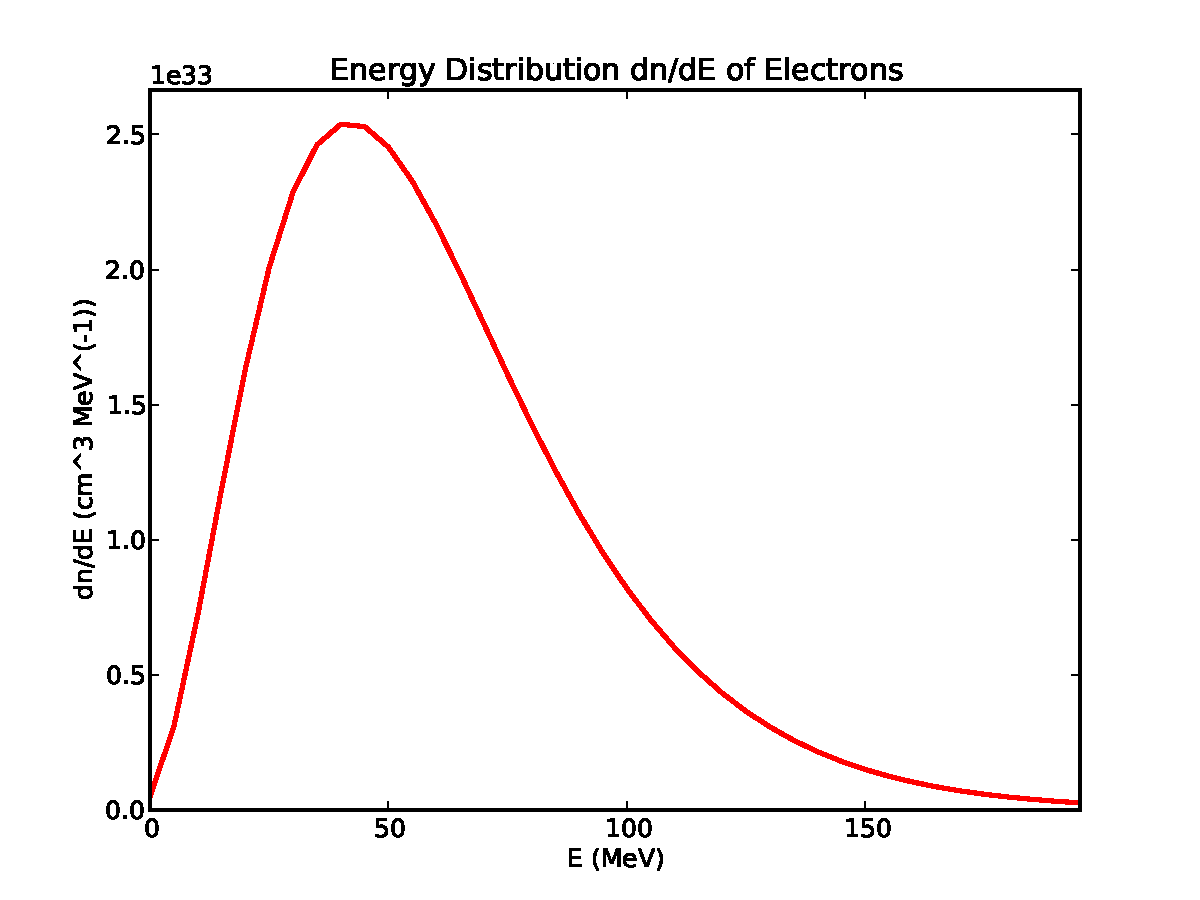
\includegraphics[width=0.5\textwidth]{gauss-legendre.pdf}
\caption{Plot of $dn_{e^{\pm}}/dE$ vs Energy in MeV}
\label{fig:legendre}
\end{figure}

We see that plotting the values of $\frac{dn_{e^{\pm}}}{dE}$ in over the 
energy bins we calculated produces a reasonable looking distribution. 
We can also confirm that 
$$ \sum\limits_{i=0}^{39} \left[ \frac{dn_{e^{\pm}}}{dE} \right]_i * \Delta E \approx n_{e^{\pm}} $$ as the infinite sum should be equal to the density. This is indeed true: python reports that the relative error of the sum 
compared to the electron density is $-0.00307178501624$.


\end{document}